\chapter{Implementação e Testes}
% Os titulos dados aos capítulos são meros exemplos. Cada relatório deve adequar-se ao projeto desenvolvido.
\label{chap:imp-test}

\section{Introdução}
\label{chap4:sec:intro}
O capítulo 4 e dedicado á apresentação de algumas funções implementadas no âmbito do projeto e também alguns testes efetuados.

\section{Implementação}
\label{chap4:sec:...}

\subsection{HTML dinâmico}
Durante o desenvolvimento deste projeto, foi usada a construção dinâmica de um ficheiro \ac{HTML}, que diz respeito a uma notícia. 

\begin{lstlisting}[language=Java, caption = Exemplo de construção de \ac{HTML} dinâmico \label{code:html_dinamico}]
String html
    = "<html>"
    + "   <head>"
    + "      <style>"
    + "         p { text-align: justify;}"
    + "      </style>"
    + "   </head>"
    + "   <body bgcolor=" + "\"" + bgcolor + "\">"
    + "      <img src=" + "\"" + imagensAtualidade.get(i) + "\"" + "align=" + img_align + " width=\"150\" height=\"130\" />"
    + "      <p><b>" + titulosAtualidade.get(i) + "</b><br>"
    + paragrafosActualidade.get(i)
    + "      </p>"
    + "   </body>"
    + "</html>";
webviewActualidade[i].getEngine().loadContent(html);    

\end{lstlisting}
Neste caso foram usados métodos de \emph{Jsoup} para extrair a informação pretendida de uma página. Essas informações são armazenadas em \emph{ArrayList<String>}, e é a partir delas que se constrói o \ac{HTML}. Estão presentes três \emph{ArrayList} diferentes, \emph{imagensAtualidade, titulosAtualidade e paragrafosAtualidade}. Cada uma armazena informações em \emph{Strings} referentes às imagens, aos títulos e aos parágrafos, das noticias. \par
No fim de a \emph{string html} estar finalizada, necessitamos de mostrar o seu conteúdo. Para isso é usado um objeto do tipo \emph{WebView}, este permite exibir uma página \emph{web}, quer através do \emph{link} direto para o mesmo ou através de uma \emph{string}, o último é usado neste projeto.
Através dos métodos \emph{getEngine().loadContent(html)} é possível carregar o conteúdo da string para o \emph{webview}, neste caso se as dimensões da página forem superiores às dimensões do \emph{webview}, este cria um \emph{scroll} automático. Esta é uma propriedade bastante interessante pois em grande parte dos casos as notícias excedem o tamanho do \emph{webview}.


\subsection{DestkNew}
Esta função determina se uma notícia vai ser ou não destacada, alterando a cor de fundo da mesma. Tem como objetivo realçar uma notícia aos olhos do utilizador. 

\begin{lstlisting}[language=JAVA, caption = Código usado para destacar notícia \label{code:imagens}]
private Boolean destakNew(String texto_noticia)
HashSet<String> textNot = new HashSet<>();
String[] palavras = texto_noticia.trim().split("[ ,;:.!?\n]+");
for (String palavra : palavras) {
    textNot.add(palavra);
}

int lexSize = lexicoRelevante.size();
textNot.retainAll(lexicoRelevante);
double conjuction = (double) textNot.size() / lexSize;

if (conjuction > 0.35) {
    return true;
} else {
    return false;
}    
\end{lstlisting}

Para isso foi usado um léxico de palavras escolhido pelo utilizador, esse léxico é comparado com o texto da notícia e no final só é destacada se a interseção dos dois conjuntos for superior a 35\%. \par
Assim sendo, são usados objetos do tipo \emph{HashSet<String>}, este cria uma estrutura de \emph{string} que usa tabelas de \emph{hash} para armazenar os dados. Não permite objetos duplicados e e não segue a ordem de inserção dos dados, cada \emph{string} é identificada com um número único. \par
Na Listing 4.2 visível o \emph{lexicoRelevante}, um \emph{HashSet} que carrega as palavras de um ficheiro. Este ficheiro é manipulado pelo utilizador e deve conter palavras que ache relevantes aparecerem na notícia. Estas vão depender do seu gosto e das suas preferências. Outro \emph{HashSet} utilizado é o \emph{textNot}, que por sua vez contem as palavras presentes no parágrafo da notícia.\par 
Através do método \emph{retainAll} é feita a interseção dos dois \emph{HashSet} e a partir daqui é possível relacionar o texto da notícia com o léxico. Este método devolve apenas o conjunto de \emph{strings} comuns nos dois conjuntos de dados. Sendo o \emph{lexSize} o tamanho do \emph{lexicoRelevenate}, usado para calcular a percentagem final de quantas palavras do léxico estão presentes na notícia.
A seguinte expressão demonstra o cálculo efetuado no algoritmo:
\begin{equation}
    \mu= \dfrac{textNot \cap lexicoRelevante}{lexSize}
\end{equation}

Se ocorrer que, \begin{equation}
    \mu>35\%
\end{equation}
a notícia será destacada. Optou-se por 35\%, pois apesar de existir um léxico para cada tema, dentro do mesmo tema podem existir várias palavras que não faz sentido aparecerem  na mesma notícia.

De seguida são demonstrados alguns exemplos, atribuindo valor a cada um dos \emph{HashSet}.
\begin{table}[H]
\centering
\begin{tabular}{|c|c||c|}
\hline
\textbf{textNot} & \textbf{lexicoRelevante} & \textbf{retainAll}\\
\hline
\hline
primeiro & economia & Costa \\
\hline
ministro & parlamento &  António\\
\hline
António &  petróleo & sucesso\\
\hline
Costa &  Angola & cimeira\\
\hline
considera &  António & ministro\\
\hline
cimeira &  Costa & europeia\\
\hline
europeia &  cimeira & primeiro\\
\hline
um  & europeia&\\
\hline
sucesso &  investimento &\\
\hline
 & orçamento & \\
\hline
\end{tabular}
\caption{Exemplo de interseção de dois léxicos.}
\label{tab:exemplo}
\end{table}

Na tabela 4.1 observamos o resultado do método \emph{retainAll}, dado dois léxicos, um com a notícia e outro com o \emph{léxicoRelevante}. Podemos concluir que a notícia presente no exemplo será destacada.


\vspace{0,07cm}
\begin{figure}[H]
\centering
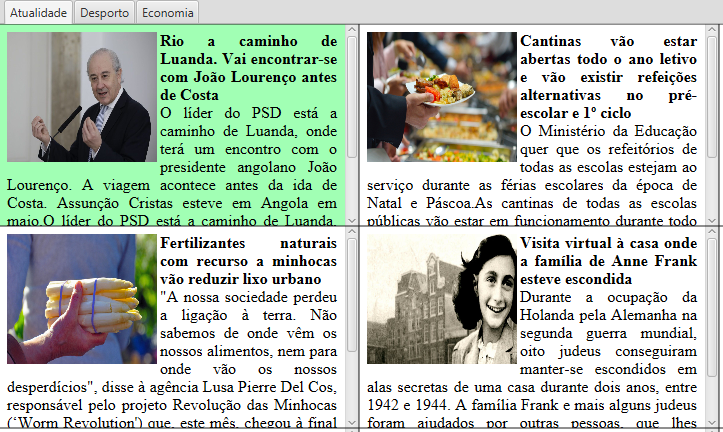
\includegraphics[scale=0.5]{imagens/new_destak.PNG}
\caption{Exemplo de notícia destacada.}
\label{fig:gestao}
\end{figure}
Na figura 4.1 é possível ver a diferença que existe para o utilizador de uma notícia que foi destacada, para as restantes. Aqui obtemos o efeito pretendido, uma vez que a notícia desperta a atenção do utilizador, sendo fácil localizar primeiro as notícias destacadas.\par



\subsection{getParagraph}
\label{chap4:sec:paragraph}
Esta função é muito relevante no contexto do projeto, uma vez que permite simplificar a notícia que será mostrada.
Para isto é usado um algoritmo bastante simples mas muito eficaz.

\begin{lstlisting}[language=JAVA, caption = Código usado para destacar notícia \label{code:getparagraph}]
Document doc = Jsoup.connect(url).get();
Elements paragrafos = doc.select("p");
StringBuilder sb = new StringBuilder();
    for (Element paragrafo : paragrafos) {
        String t = paragrafo.text().trim();
        if (t.length() == 0) {
                continue;
        }
        char last = t.charAt(t.length() - 1);
        if (".!?".contains(last + "")) {
            sb.append(t);
            if (sb.length() > 200) {
                    break;
            }
        }
    }
\end{lstlisting}
Com recurso a \emph{Jsoup} escolhe-se o primeiro parágrafo, \emph{p}, do documento \ac{HTML}. O próximo passo é escolher apenas aqueles cujo último caráter seja um dos seguintes sinais de pontuação: ., ! ou ?.
Este algoritmo é simples mas extremamente eficaz, uma vez que todos os parágrafos de uma notícia terminam com alguns destes sinais de pontuação, neste caso será guardado o primeiro parágrafo por ser considerado o que contem informações mais relevantes dentro de uma notícia. Esta seleção de parágrafos mostrou-se importante, uma vez que algumas páginas \emph{web} não usam as \emph{tags p} para mostrar os parágrafos da notícia, houve casos em que o primeiro parágrafo do \emph{website} dizia respeito ao autor do texto e não propriamente do texto da notícia.

\section{Conclusões}
\label{chap4:sec:concs}
Neste capítulo foram apresentadas algumas funções usadas, bem como o resultado da sua utilização. 